\documentclass{article} 
	\usepackage{graphicx}
	\usepackage{geometry}
	\geometry{a4paper,left=1cm,right=1cm,top=2cm,bottom=2cm}
   	\author{Yifan Xu 22605382} 
   	\title{EECS 112L Lab3 Report} 
\begin{document}
	\maketitle
	\section{Block Diagram}
	\subsection{Block Diagram} 
	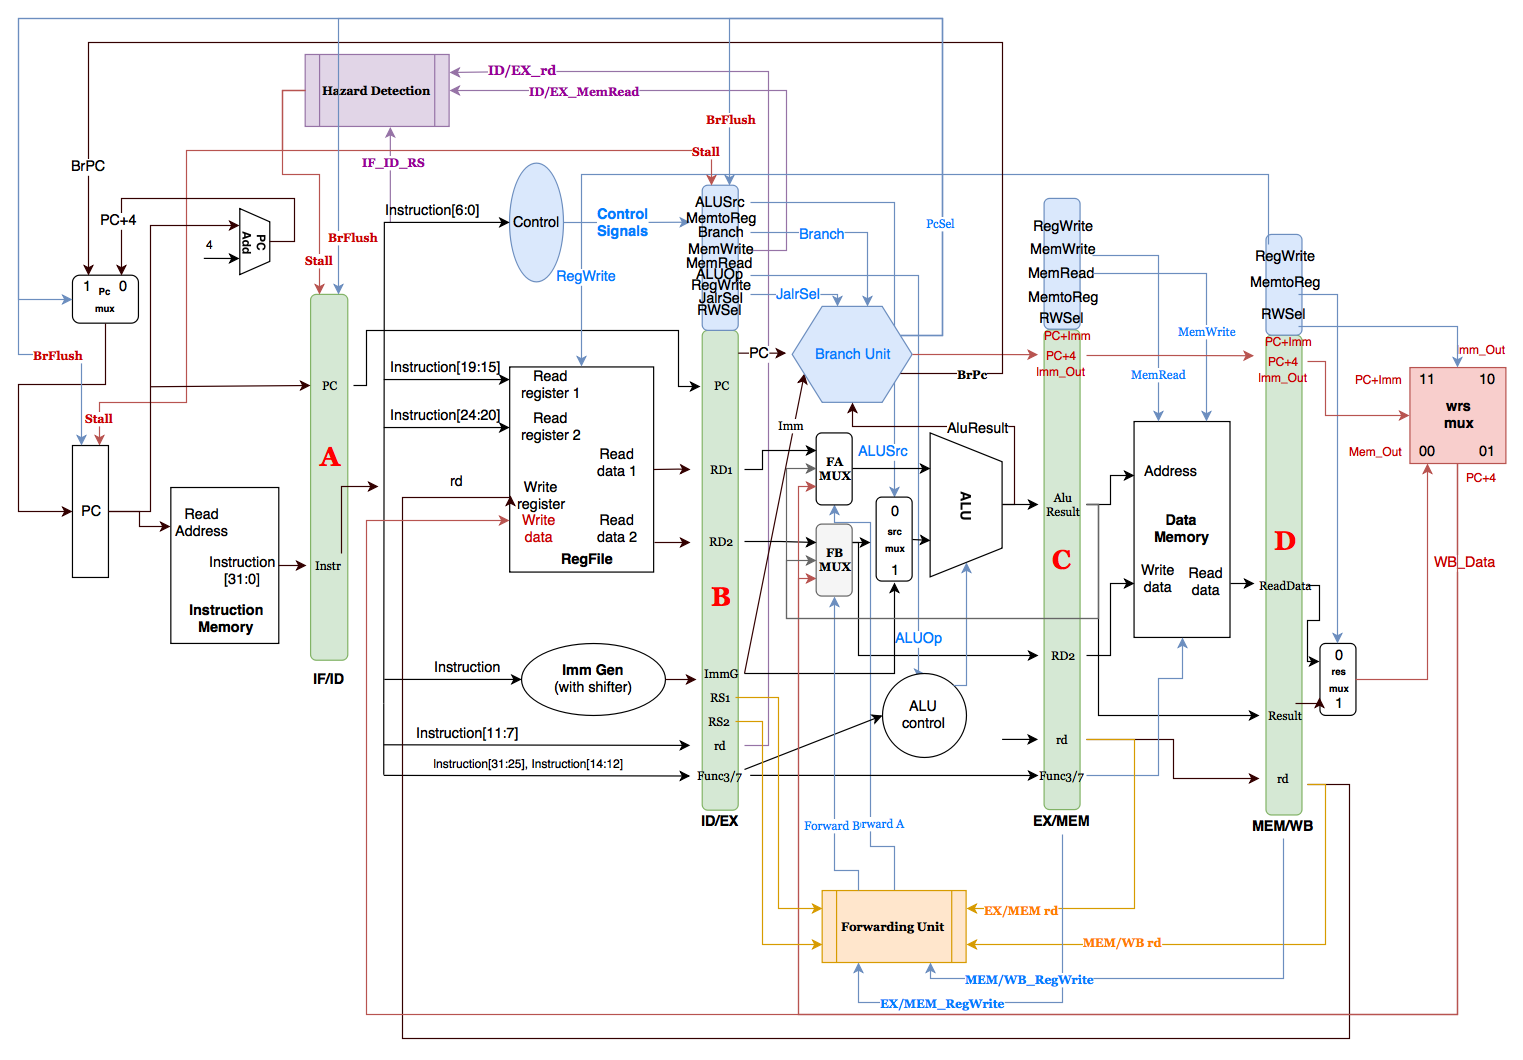
\includegraphics[scale=0.37]{PipeLine.png}
	\section{Detailed Explanation}
	\subsection{Initialization}
	To realize Pipeline idea, we introduce four buffer register between each stage.
	\paragraph{Register A} Register between IF and ID stage
	\paragraph{Register B} Register between ID and EX stage
	\paragraph{Register C} Register between EX and MEM stage
	\paragraph{Register D} Register between MEM and WB stage \\ \\
	All four Buffer Registers will be updated at positive edge of clock signal. Also, at the very beginning, which refers to the positive edge of reset signal, major elements in all 4 registers will be set to 0 as initialization.
	\subsection{Instruction Fetch Stage} 
	\subsubsection{Instruction Memory} 
	In this stage, Instruction Memory will fetch specific instruction code according to the value generated by PC. Then, at the positive edge of the following clock cycle, this instruction will be written to the Register A so that new instruction code could be fetched.
	\subsubsection{Next-PC-Select Mux}
	A 2-to-1 mux controls the value that should be used for fetching instruction in the next clock cycle. The first option is current PC+4. the second option is the generated PC value from Branch Unit. Only when branch is taken will this option be selected. The mux control also comes from Branch Unit. (See 2.4.1 for more information) 
	\subsection{Instruction Decode Stage}
	In this stage, instruction code acquired from Register A will be divided into different chunks and used by Controller, Imm-Generator and Reg-File. The logic is the same as what we did in single cycle project. However, instead of connecting those controls and read data directly to different operation units, we storing them in Register B for further usage.
	\subsection{Execution Stage}
	In this stage, we use the data and control signals in Register B to drive Branch Unit and ALU. \textbf{Note, dislike what we set in Lab2, the ALUOp signal in Pipeline processor comes from Register B. Therefore, ports definition of ALU Controller in RISC-V.sv is changed.}
	\subsubsection{Branch Unit}
	The new designed Branch Unit is charged of calculation next PC value if branch instruction was fetched in IF stage. If JALR or JAL or BRANCH instruction is taken, output PcSel will be set to 1. \\
	As to new PC value (output BrPc), it will be set to \underline{PC+Imm} if BRANCH/JAL is taken or \underline{AluResult} if JALR is taken. \\
	Both BrPC and PcSel will be directly connected to PcSel mux. That means, whenever Branch Unit finish its job, the PC Select mux gets all what it needs. However, the processor still need to wait until the next positive edge to do the actual select.
	Therefore, according to my design, each taken branch instruction will need to flush 2 pre-processed instructions ahead in IF and ID stage at that moment. (See 2.7 for more information about "flush")
	\subsubsection{ALU with Forwarding}
	Two forwarding select muxs are added to ALU SrcA and SrcB. If no hazard, mux will select \underline{RD1} and \underline{RD2} from Register B. If EX hazard happens, mux will select \underline{AluResult} for either SrcA or SrcB. If MEM hazard happens, mux will select \underline{WB-Data} for either SrcA or SrcB. 
	\subsection{Memory Operation Stage}
	The logic in this stage is the same as the single cycle processor. However, the control signals and data comes from Register C instead.
	\subsection{Data Write Back Stage}
	In this section, a 4 to 1 mux will select the right signal that should be write back to register file, if write back is required. \textbf{Note, if a flushed instruction enter this stage, the signal \underline{WB-Data} may still have trash value, but means nothing, and will not affect RegFile.}
	\subsection{Hazard Detection Unit}
	A Hazard Detection Unit is added to pipeline datapath. If data dependency hazard is detected, a stall signal will be generated to PC, Register A and Register B.
	PC check stall signal every clock positive edge. Whenever this signal has value 1, PC output will be set to 9'b0 instead of next PC value to simulate a NOP instruction.
	Register A and B check stall signal every clock positive edge. Whenever this signal has value 1, Register will empty all data stored inside to avoid trash data entering next stage, which also functions like a NOP instruction.
	\subsection{Register Flush Signal}
	The Flush Signal functions in the same way as Stall signal in PC, Register A and Register B, but generated by Branch Unit. The purpose of having this signal is to flush wrong instructions, which was fetched and executed before any taken BRANCH instruction.
	
	\section{Waveform}
	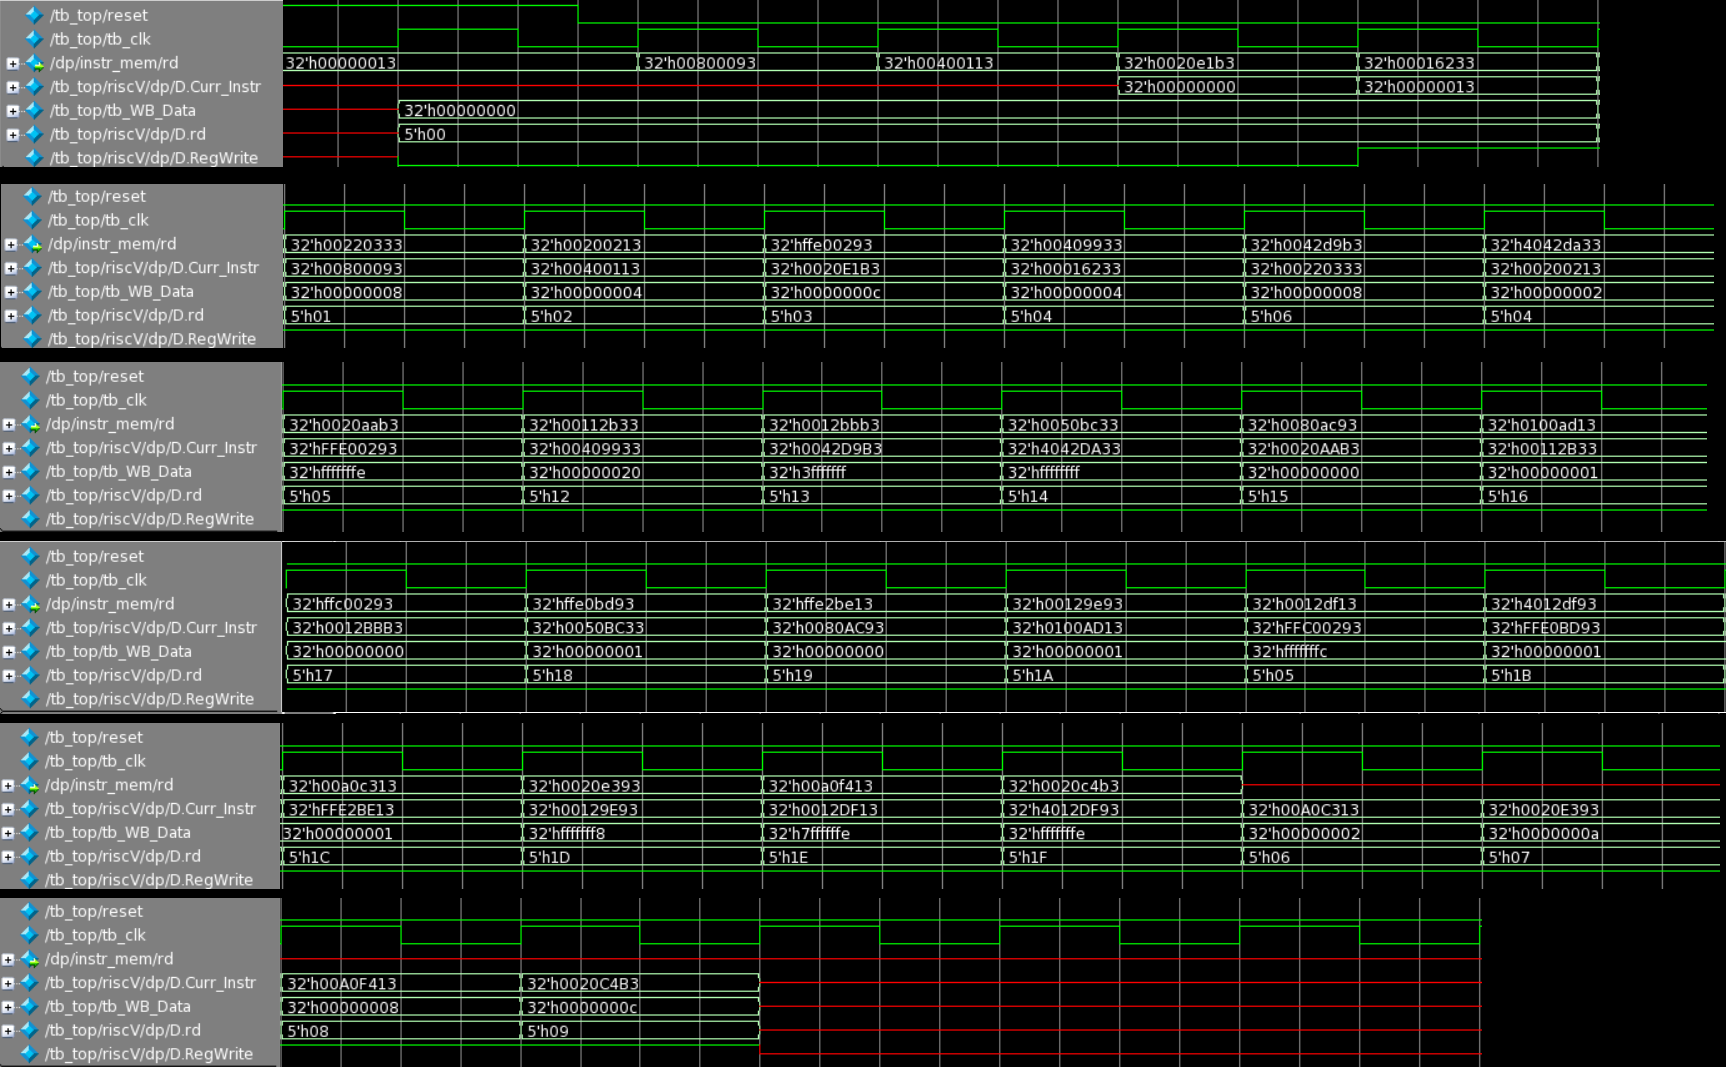
\includegraphics[scale=0.65]{WaveForm.png}
	\section{Synthesis Report}
	\subsection{Critical Path}
	\paragraph{Critical Path Length} 3.07
	\paragraph{Critical Path Slack}  0.92\\
  Timing Path Group 'clk'\\
  -----------------------------------\\
  Levels of Logic:              44.00\\
  Critical Path Length:          3.07\\
  Critical Path Slack:           0.92\\
  Critical Path Clk Period:      4.00\\
  Total Negative Slack:          0.00\\
  No. of Violating Paths:        0.00\\
  Worst Hold Violation:          0.00\\
  Total Hold Violation:          0.00\\
  No. of Hold Violations:        0.00\\
  -----------------------------------\\
	\subsection{Area}
Area\\
  -----------------------------------\\
  Combinational Area:     9063.029220\\
  Noncombinational Area:  8059.160647\\
  Buf/Inv Area:            663.315843\\
  Total Buffer Area:           291.25\\
  Total Inverter Area:         372.07\\
  Macro/Black Box Area:      0.000000\\
  Net Area:               6016.975920\\
  -----------------------------------\\
  Cell Area:             17122.189867\\
  Design Area:           23139.165787\\
	\subsection{Power}
	\includegraphics[scale=0.8]{power.png}
	\subsection{Comparison}
	For Single Cycle:\\
	Critical Path Length 5.31\\
	Critical Path Slack -3.34\\
	======================\\
	Pipeline Design has shorter critical path and more efficient performance.
	\end{document}